\documentclass{standalone}
\usepackage{tikz}
\usepackage{amsmath}
\usetikzlibrary{decorations.pathreplacing}

\begin{document}
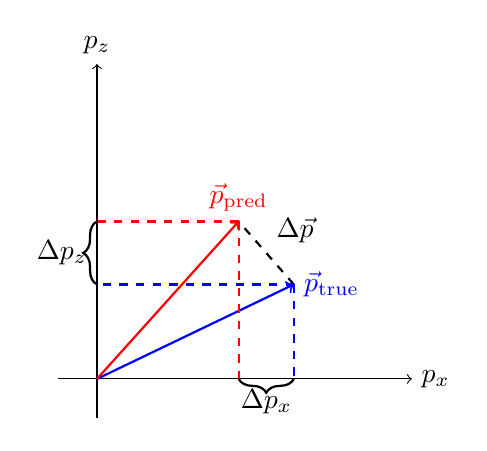
\begin{tikzpicture}[scale=1]


    % Axes
    \draw[->] (-0.5,0) -- (4,0) node[right] {$p_x$};
    \draw[->] (0,-0.5) -- (0,4) node[above] {$p_z$};

    \coordinate (origin) at (0,0);
    \coordinate (true) at (2.5,1.2);
    \coordinate (pred) at (1.8,2.0);
    \coordinate (true_x) at (2.5,0);
    \coordinate (true_z) at (0,1.2);
    \coordinate (pred_x) at (1.8,0);
    \coordinate (pred_z) at (0,2.0);

    % True vector
    \draw[thick,blue,->] (origin) -- (true) node[right] {$\vec{p}_{\text{true}}$};
    % Predicted vector
    \draw[thick,red,->] (origin) -- (pred) node[above] {$\vec{p}_{\text{pred}}$};

    % Loss vector
    \draw[thick,dashed] (true) -- (pred) node[midway, above right] {$\Delta \vec p$};

    % show x and z projections
    \draw[thick,blue,dashed] (true) -- (true_x);
    \draw[thick,blue,dashed] (true) -- (true_z);
    \draw[thick,red,dashed] (pred) -- (pred_x);
    \draw[thick,red,dashed] (pred) -- (pred_z);
    \draw[decorate,decoration={brace,amplitude=5pt}, thick] (true_x) -- (pred_x) node[midway,below] {$\Delta p_x$};
    \draw[decorate,decoration={brace,amplitude=5pt}, thick] (true_z) -- (pred_z) node[midway,left] {$\Delta p_z$};

\end{tikzpicture}

\end{document}